\documentclass[a4paper,11pt]{article}

% Use utf-8 encoding for foreign characters
\usepackage[utf8]{inputenc}
\usepackage[british,english]{babel}
\usepackage[T1]{fontenc}

% Setup for fullpage use
\usepackage{fullpage}

% Multipart figures
\usepackage{subfigure}

% More symbols
\usepackage{amsmath}
\usepackage{amssymb}
\usepackage{latexsym}

\usepackage{booktabs}

% For pretty URLs, see: http://en.wikibooks.org/wiki/LaTeX/Hyperlinks
\usepackage{hyperref}

% Surround parts of graphics with box
\usepackage{boxedminipage}

% Package for including code in the document
\usepackage{listings}

% If you want to generate a toc for each chapter (use with book)
\usepackage{minitoc}

% Uncomment if you want to use Palatino as font
\usepackage[sc]{mathpazo}
\linespread{1.05}         % Palatino needs more leading (space between lines)

% This is now the recommended way for checking for PDFLaTeX:
\usepackage{ifpdf}

% Used for highlighting text with \hl{}
\usepackage{soul}

\addto\captionsenglish{\renewcommand{\refname}{}}

%\newif\ifpdf
%\ifx\pdfoutput\undefined
%\pdffalse % we are not running PDFLaTeX
%\else
%\pdfoutput=1 % we are running PDFLaTeX
%\pdftrue
%\fi

\ifpdf
\usepackage[pdftex]{graphicx}
\else
\usepackage{graphicx}
\fi
\title{Deliverable 7: Sprint \#5\\\small{for}\\\small{Danske Bank: Peer-to-peer}}
\author{ Group Delta:\\Jesper Borgstrup, Thomas Kjeldsen and Mads Ohm Larsen }

\date{June 10, 2011}

\begin{document}

\ifpdf
\DeclareGraphicsExtensions{.pdf, .jpg, .tif}
\else
\DeclareGraphicsExtensions{.eps, .jpg}
\fi

\maketitle


\pagebreak

%\tableofcontents
%\vspace{2cm}

%%%%%%%%%%%%%%%%%%%%%%%%%%%%%%%%%%%%%%
%%%%%%%%%%%%%%%%%%%%%%%%%%%%%%%%%%%%%%
%%%%%%%%%%%%%%%%%%%%%%%%%%%%%%%%%%%%%%

\section{Requirements for this deliverable}
\begin{enumerate}
\item Doing a demo in class (on 2011-05-18)
\item Giving us access to your source code
\item Handing in a collection of your sprint material
\item Describing a sprint retrospective (e.g., as a set of bullets outlining what
when well, what went wrong, and how you will improve for the next sprint)
\item Description of process improvement efforts
\end{enumerate}

The Sprint Demo was given on June 8th. This document describes requirements 2-4 as well as the sprint learning goal -- reflection on and improvement of our software development process.

%%%%%%%%%%%%%%%%%%%%%%%%%%%%%%%%%%%%%%
%%%%%%%%%%%%%%%%%%%%%%%%%%%%%%%%%%%%%%
%%%%%%%%%%%%%%%%%%%%%%%%%%%%%%%%%%%%%%


%%%%%%%%%%%%%%%%%%%%%%%%%%%%%%%%%%%%%%
%%%%%%%%%%%%%%%%%%%%%%%%%%%%%%%%%%%%%%
%%%%%%%%%%%%%%%%%%%%%%%%%%%%%%%%%%%%%%

\section{Source code access}
Our source code is publicly available on GitHub from \url{https://github.com/omegahm/DBP2P}.

If you wish to checkout our code (read-only) using Git, then use git clone with this URL:
\url{git://github.com/omegahm/DBP2P.git}

The code used for our presentation is stored as commit \href{https://github.com/omegahm/DBP2P/commit/d120c1657b8c1582d8357cbba3efcc10332a71e5}{d120c16...71e5}.

The introduction and guide to using the library (README.md) can be viewed at \href{https://github.com/omegahm/DBP2P}{https://github.com/omegahm/DBP2P}.

%%%%%%%%%%%%%%%%%%%%%%%%%%%%%%%%%%%%%%
%%%%%%%%%%%%%%%%%%%%%%%%%%%%%%%%%%%%%%
%%%%%%%%%%%%%%%%%%%%%%%%%%%%%%%%%%%%%%

\section{Sprint material}
Sprint Material needed to assess our progress include the following:
\begin{itemize}
\item source code (version number and access method is sufficient)
\item product backlog (before and after the sprint)
\item sprint backlog
\item any other material (e.g., burndown chart) that illustrates your progress
\end{itemize}

\subsection{Sprint Backlog}
Our sprint backlog is shown in figure \ref{sprintbacklog} on page \pageref{sprintbacklog}.

  \begin{figure}[ht!]
  	\begin{center}
  	% Insert sprint backlog here
  	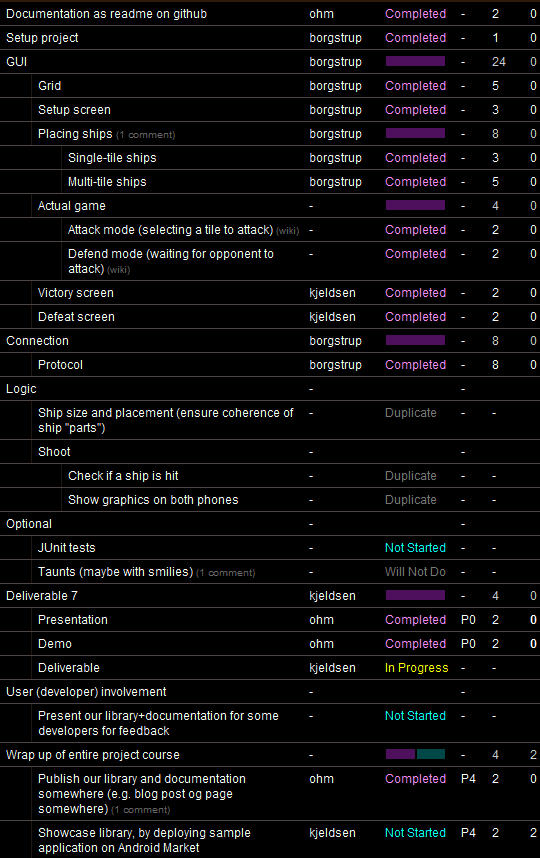
\includegraphics[width=0.85\textwidth]{sprint_backlog.png}		
  	\end{center}
  	\caption{Our sprint backlog after the sprint was finished}
  	\label{sprintbacklog}
  \end{figure}

\subsection{Burndown chart}

Our burndown chart is shown in figure \ref{burndown} on page \pageref{burndown}.

  \begin{figure}[ht!]
  	\begin{center}
  	% Insert burndown chart here
  	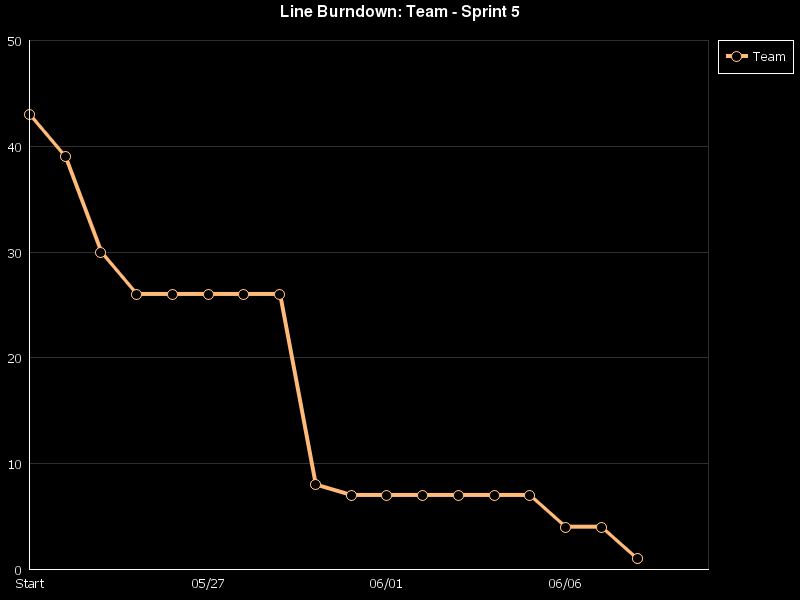
\includegraphics[width=\textwidth]{line_burndown.png}		
  	\end{center}
  	\caption{Our burndown chart at the end of the sprint}
  	\label{burndown}
  \end{figure}

%\subsection{Acunote}
%We have got an Acunote account\footnote{\url{http://dbp2p.acunote.com/}} setup, and %access to this have been granted.
%
%\clearpage
%
%%%%%%%%%%%%%%%%%%%%%%%%%%%%%%%%%%%%%%
%%%%%%%%%%%%%%%%%%%%%%%%%%%%%%%%%%%%%%
%%%%%%%%%%%%%%%%%%%%%%%%%%%%%%%%%%%%%%

\clearpage

\section{Sprint retrospective}

What went well during this sprint:

\begin{itemize}
\item Early start of development
\item Good idea for sample application
\item Motivated development
\end{itemize}

\noindent
What went wrong:
\begin{itemize}
\item Nothing
\end{itemize}

\noindent
How we will improve:
\begin{itemize}
\item We’ll do further reflection during the exam, when course has been fully concluded
\end{itemize}

\section{Process improvement}

Discussing our past retrospectives yielded some useful info which used to generate the FRIM chart seen in figure \ref{frim} on page \pageref{frim}.

\begin{figure}
	\centering
	\begin{tabular}{|c|p{3cm}|p{3cm}|p{3cm}|p{3cm}|}
	\hline
		& Once & Several times & Often & All the time \\\hline
	+2  & & & Skype meetings \par\vspace{.3cm} Demos & Acunote tool for Scrum \\\hline
	+1  & & Product owner meetings & Coherent breakdown of tasks with time estimates \par\vspace{.3cm} Lectures & Use of shared calendar \par\vspace{.3cm} Git as configuration management tool \\\hline
	 0  & Code inspection with other team & & Virtual scrum meetings & \\\hline
	-1  & & Communication hickups & User stories & \\\hline
	-2  & Easter holiday & Forced re-definement of project scope \par\vspace{.3cm} Underestimation of task workload & Majority of work was postponed to end of sprint & \\\hline
	\end{tabular}	
	\caption{FRIM}
	\label{frim}
\end{figure}

We then generated the AB Matrix seen in figure \ref{abmatrix} on page \pageref{abmatrix}, however with only 3 team members we did not split up into two teams (A and B) which is why our matrix is really just a vector.

\begin{figure}
	\centering
	\begin{tabular}{|p{3cm}|p{3cm}|p{3cm}|p{3cm}|}
	\hline
	What is working? \par What is right? & What is good behaviour? & What is not quite working yet? & What does the ideal situation look like? \tabularnewline\hline

	Acunote tool for tracking Scrum process
	\par\vspace{.5cm}
	Good working environment
	\par\vspace{.5cm}
	Stories/Projects broken down in to doable and manageable tasks
	\par\vspace{.5cm}
	Time estimation of work
	\par\vspace{.5cm}
	Sharing of knowledge
	(Scrum, Git, calendar)
	\par\vspace{.5cm}
	FRIM grid, AB matrix

	& 

	Being on time
	\par\vspace{.5cm}
	Do work
	\par\vspace{.5cm}
	Regularly communicating status and problems to other team members and involve them in overcoming obstacles
	\par\vspace{.5cm}
	Writing tests, then code
	\par\vspace{.5cm}
	Well planned demo, with backup plan
	
	& 
	
	Tests
	\par\vspace{.5cm}
	Starting early rather than having workload pile up towards the end of sprint
	\par\vspace{.5cm}
	Keeping focus VS distractions/low priority tasks
	\par\vspace{.5cm}
	No backup plan for demo
	
	& 
	
	Everybody on the team knows what to do, when to do it, and actually does it
	\par\vspace{.5cm}
	Good sharing of knowledge
	(Scrum, Git, calendar)
	\par\vspace{.5cm}
	Clearly defined goal(s) from the beginning
	\tabularnewline\hline
	\end{tabular}	
	\caption{AB Matrix}
	\label{abmatrix}
\end{figure}

Finally we decided how to address this in this sprint; the results of which can be seen in figure \ref{whattodo} on page \pageref{whattodo}.

  \begin{figure}[ht!]
  	\begin{center}
  	% Insert burndown chart here
  	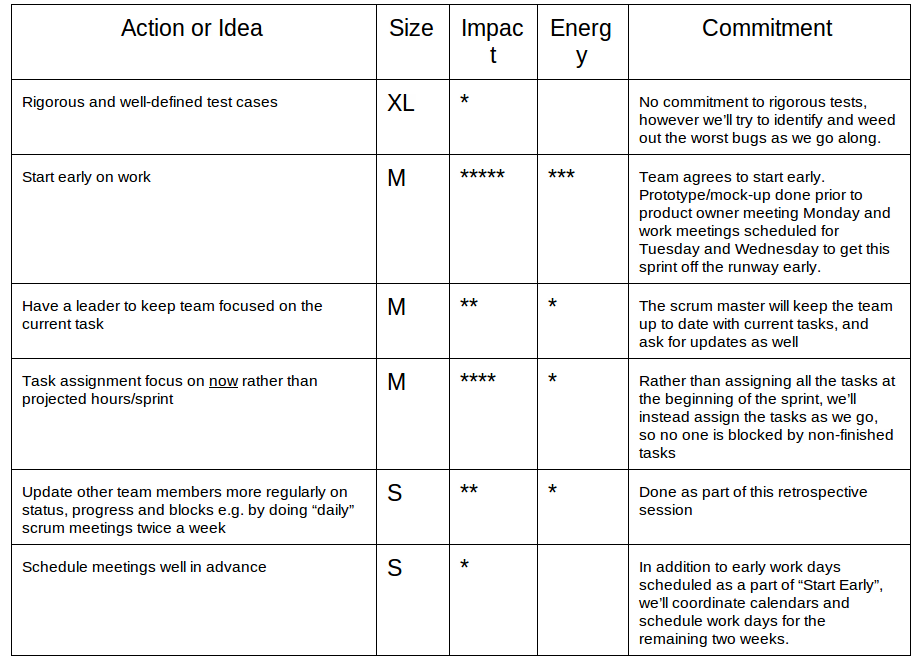
\includegraphics[width=\textwidth]{whattodo.png}		
  	\end{center}
  	\caption{What to do}
  	\label{whattodo}
  \end{figure}

\end{document}
